\aufgabe{Counterfactuals - Image Data}
{
	A wildlife conservation organisation uses a machine learning model to classify animals in camera-trap images.
	The following image was classified as a lynx.
	
	\begin{figure}[H]
		\centering
		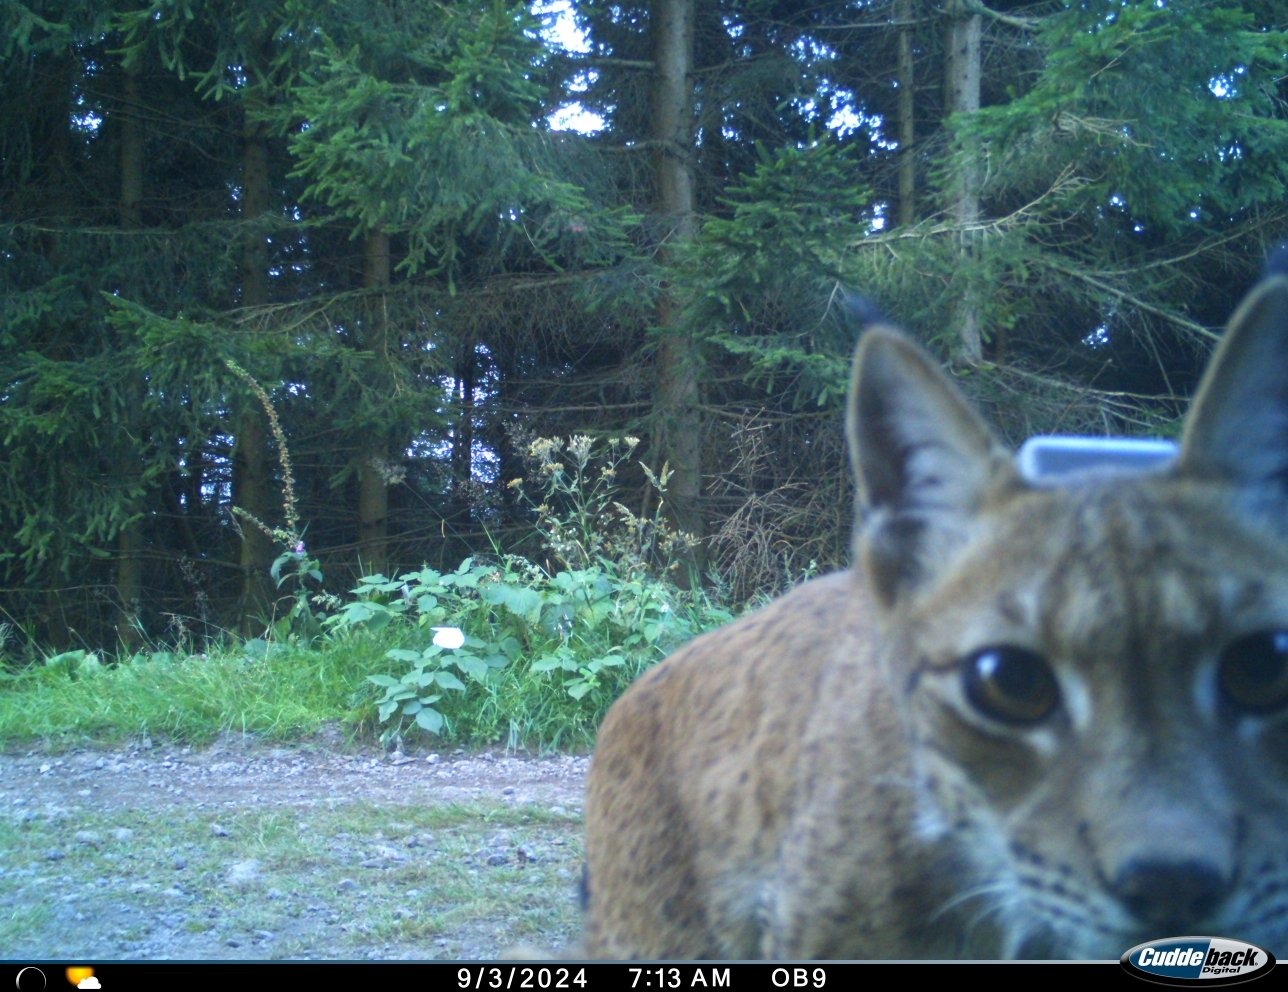
\includegraphics[width = .43\textwidth]{ex_tex/lynx_image}
		\caption{Image from \href{https://www.wildnispark.ch/en/general/news/lynx-vreni-from-wildnipark-zurich-has-settled-in-well-in-germany-655}{Wildnispark Zürich}}
	\end{figure}
	
	\noindent Researchers generate the following counterfactual explanations:
	
	\begin{itemize}
		\item[CE1]
		``If the spotted fur pattern were less visible and the nose would be smaller and more pointed, the image would have been classified as a fox.''
		
		\item[CE2]	``If the background vegetation were greener and denser, the image would have been classified as a fox.''
		
		\item[CE3]	``If several pixels across the image were modified in a way nearly invisible to humans, the image would have been classified as a deer.''
		
		\item[CE4] 	``If the timestamp watermark were removed, the image would have been classified as a fox.''
		
	\end{itemize}
	
	
	Discuss the following in groups: 
	\begin{enumerate}[a)]
		
		\item Which counterfactual(s) appear(s) biologically plausible?
		
		\textcolor{blue}{CE1 because it reflects biological characteristics that clearly separate a lynx from a fox.}
		
		\item Which counterfactual(s) reflects that our model is not robust?
		
		\textcolor{blue}{CE3 reflects this the most but also CE2 and CE4 are less robust, slight changes in the background or removal of the watermark should not change the prediction}
		
		\item Which counterfactual(s) suggest(s) the model may rely on spurious association?
		
		\textcolor{blue}{CE2 and CE4, changes in the background or removal of the watermark change the prediction but these are not characteristics of the lynx}
		
		\item What does counterfactual CE4 suggest about the dataset or data collection process?
		
		\textcolor{blue}{(Many of the) lynx images contain watermarks but fox images do not (or not as many)}
		
		\item Which counterfactual(s) would concern you most as a machine learning engineer?
		
		\textcolor{blue}{CE2 to CE4. CE2 and CE3 reflect that the model does not learn what we intend to learn, we aim for a classifier for animals not a background or watermark detector. CE4 reflects that our model is not robust.}
		
		\item Are any of these counterfactuals actionable? If yes, for whom?
		
		\textcolor{blue}{The aim of the counterfactuals is not recourse (reverting a classification), consequently, actionability of the counterfactual should not be an objective for finding counterfactuals.}
		
	\end{enumerate}
}
